% SIAM Article Template
\documentclass[review,onefignum,onetabnum]{siamonline250106}

\usepackage{caption}
\captionsetup{compatibility=false}
% Information that is shared between the article and the supplement
% (title and author information, macros, packages, etc.) goes into
% ex_shared.tex. If there is no supplement, this file can be included
% directly.

% SIAM Shared Information Template
% This is information that is shared between the main document and any
% supplement. If no supplement is required, then this information can
% be included directly in the main document.


% Packages and macros go here
\usepackage{lipsum}
\usepackage{amsfonts}
\usepackage{graphicx}
\usepackage{epstopdf}
\usepackage{soul}
\usepackage{caption}
\usepackage{subcaption}
\usepackage{algorithm}
\usepackage{algpseudocode}
\usepackage{enumitem}
\usepackage{comment}
\ifpdf
  \DeclareGraphicsExtensions{.eps,.pdf,.png,.jpg}
\else
  \DeclareGraphicsExtensions{.eps}
\fi

% \usepackage[dvipsnames,x11names]{xcolor}

\usepackage{booktabs}
\usepackage{multirow}
\usepackage{annotate-equations}

% Prevent itemized lists from running into the left margin inside theorems and proofs
\usepackage{enumitem}
\setlist[enumerate]{leftmargin=.5in}
\setlist[itemize]{leftmargin=.5in}

% Add a serial/Oxford comma by default.
\newcommand{\creflastconjunction}{, and~}

% Used for creating new theorem and remark environments
\newsiamremark{remark}{Remark}
\newsiamremark{hypothesis}{Hypothesis}
\crefname{hypothesis}{Hypothesis}{Hypotheses}
\newsiamthm{claim}{Claim}

% Sets running headers as well as PDF title and authors
% \headers{Utilizing Covariance Uncertainty in Multi-fidelity Estimation with Approximate Control Variates}{T. Coons, A. Jivani, and X. Huan}

\headers{Multifidelity SVGD}{A. Jivani, T. Coons and X. Huan}

% Title. If the supplement option is on, then "Supplementary Material"
% is automatically inserted before the title.
% \title{Utilizing Covariance Uncertainty in Multi-fidelity Estimation with Approximate Control Variates\thanks{Submitted to the editors DATE.
% \funding{Enter funding sources!}}}
\title{Scalable Stein Variational Gradient Descent via Multifidelity Particle Transport with Application to Bayesian Inference\thanks{Submitted to the editors DATE.
\funding{This work is supported in part by the National Science Foundation Graduate Research Fellowship under Grant No. DGE 1841052, the Department of Navy award N00014-23-1-2735 issued by the Office of Naval Research, and through computational resources and services provided by Advanced Research Computing at the University of Michigan, Ann Arbor.}}}

% Authors: full names plus addresses.
\author{Aniket Jivani\thanks{Department of Mechanical Engineering, University of Michigan, Ann Arbor, MI 48109 
  (\email{ajivani@umich.edu}, \url{https://me.engin.umich.edu/}).}
\and Thomas E. Coons\footnotemark[2]
\and Xun Huan\footnotemark[2]}

\usepackage{amsopn}
\DeclareMathOperator{\diag}{diag}


%%%% HELPER CODE FOR DEALING WITH EXTERNAL REFERENCES ON OVERLEAF
% (from an answer by cyberSingularity at http://tex.stackexchange.com/a/69832/226)
%%%
\makeatletter
\newcommand*{\addFileDependency}[1]{% argument=file name and extension
  \typeout{(#1)}% latexmk will find this if $recorder=0 (however, in that case, it will ignore #1 if it is a .aux or .pdf file etc and it exists! if it doesn't exist, it will appear in the list of dependents regardless)
  \@addtofilelist{#1}% if you want it to appear in \listfiles, not really necessary and latexmk doesn't use this
  \IfFileExists{#1}{}{\typeout{No file #1.}}% latexmk will find this message if #1 doesn't exist (yet)
}
\makeatother

\newcommand*{\myexternaldocument}[1]{%
    \externaldocument{#1}%
    \addFileDependency{#1.tex}%
    \addFileDependency{#1.aux}%
}
%%% END HELPER CODE

%%% Local Variables: 
%%% mode:latex
%%% TeX-master: "ex_article"
%%% End: 



% % SIAM Shared Information Template
% % This is information that is shared between the main document and any
% % supplement. If no supplement is required, then this information can
% % be included directly in the main document.


% % Packages and macros go here
% \usepackage{lipsum}
% \usepackage{amsfonts}
% \usepackage{graphicx}
% \usepackage{epstopdf}
% \usepackage{algorithmic}
% \ifpdf
%   \DeclareGraphicsExtensions{.eps,.pdf,.png,.jpg}
% \else
%   \DeclareGraphicsExtensions{.eps}
% \fi

% % Prevent itemized lists from running into the left margin inside theorems and proofs
% \usepackage{enumitem}
% \setlist[enumerate]{leftmargin=.5in}
% \setlist[itemize]{leftmargin=.5in}

% % Add a serial/Oxford comma by default.
% \newcommand{\creflastconjunction}{, and~}

% % Used for creating new theorem and remark environments
% \newsiamremark{remark}{Remark}
% \newsiamremark{hypothesis}{Hypothesis}
% \crefname{hypothesis}{Hypothesis}{Hypotheses}
% \newsiamthm{claim}{Claim}

% % Sets running headers as well as PDF title and authors
% \headers{Multi-fidelity SVGD}{A. Jivani, T. Coons, X. Huan}

% % Title. If the supplement option is on, then "Supplementary Material"
% % is automatically inserted before the title.
% % \title{An Example Article\thanks{Submitted to the editors DATE.
% % \funding{This work was funded by the Fog Research Institute under contract no.~FRI-454.}}}

% \title{Scalable Stein Variational Gradient Descent via Multifidelity Particle Transport with Application to Bayesian Inference\thanks{Submitted to the editors DATE.
% \funding{This work is supported in part by the National Science Foundation Graduate Research Fellowship under Grant No. DGE 1841052, the Department of Navy award N00014-23-1-2735 issued by the Office of Naval Research, and through computational resources and services provided by Advanced Research Computing at the University of Michigan, Ann Arbor.}}}

% % Authors: full names plus addresses.
% \author{Aniket Jivani \thanks{Department of Mechanical Engineering, University of Michigan, Ann Arbor, MI, 48109 
%   (Correspondence: \email{ajivani@umich.edu}).}
% \and Thomas E. Coons \footnotemark[2]
% \and Xun Huan \footnotemark[2]}

% \usepackage{amsopn}
% \DeclareMathOperator{\diag}{diag}


% %%%% HELPER CODE FOR DEALING WITH EXTERNAL REFERENCES ON OVERLEAF
% % (from an answer by cyberSingularity at http://tex.stackexchange.com/a/69832/226)
% %%%
% \makeatletter
% \newcommand*{\addFileDependency}[1]{% argument=file name and extension
%   \typeout{(#1)}% latexmk will find this if $recorder=0 (however, in that case, it will ignore #1 if it is a .aux or .pdf file etc and it exists! if it doesn't exist, it will appear in the list of dependents regardless)
%   \@addtofilelist{#1}% if you want it to appear in \listfiles, not really necessary and latexmk doesn't use this
%   \IfFileExists{#1}{}{\typeout{No file #1.}}% latexmk will find this message if #1 doesn't exist (yet)
% }
% \makeatother

% \newcommand*{\myexternaldocument}[1]{%
%     \externaldocument{#1}%
%     \addFileDependency{#1.tex}%
%     \addFileDependency{#1.aux}%
% }
% %%% END HELPER CODE

% %%% Local Variables: 
% %%% mode:latex
% %%% TeX-master: "ex_article"
% %%% End: 


% Optional PDF information
\ifpdf
\hypersetup{
  pdftitle={Scalable Stein Variational Gradient Descent via Multifidelity Particle Transport with Application to Bayesian Inference},
  pdfauthor={A. Jivani, T. Coons, and X. Huan}
}
\fi

% The next statement enables references to information in the
% supplement. See the xr-hyperref package for details.

%% Use \myexternaldocument on Overleaf
\myexternaldocument{ex_supplement}

% FundRef data to be entered by SIAM
%<funding-group>
%<award-group>
%<funding-source>
%<named-content content-type="funder-name"> 
%</named-content> 
%<named-content content-type="funder-identifier"> 
%</named-content>
%</funding-source>
%<award-id> </award-id>
%</award-group>
%</funding-group>

% \documentclass[12pt]{article}
% \usepackage{graphicx} % Required for inserting images
% \usepackage[utf8]{inputenc}

%%% tikz & libraries
\usepackage{tikz}
\usepackage{multirow}
\usetikzlibrary{backgrounds}
\usetikzlibrary{arrows,shapes}
\usetikzlibrary{tikzmark} % for \tikzmarknode
% \usetikzlibrary{calc} % for computing the midpoint between two nodes, e.g. at ($(p1.north)!0.5!(p2.north)$) 

% Commands for Highlighting text -- non tikz method
\newcommand{\highlight}[2]{\colorbox{#1!17}{$#2$}}
\newcommand{\highlightdark}[2]{\colorbox{#1!47}{$#2$}}
%%% NOTE: \colorbox sets the second argument in text mode, so for use within equations we wrap it in $ $ again
% if you use \highlight or \highlightdark in subscripts, you need to pass \scriptstyle to get the font size right
% e.g. $ \mathbb{E}_{\highlight{BurntOrange}{\scriptstyle y}} $
\usepackage{annotate-equations}

% Colors that are more readable for comments
\definecolor{darkred}{rgb}{.7,0,0}
\newcommand\Red[1]{\textcolor{darkred}{#1}}
\definecolor{darkgreen}{rgb}{.15,.55,0}
\newcommand\Green[1]{\textcolor{darkgreen}{#1}}
\definecolor{darkblue}{rgb}{0,0,0.7}
\newcommand\Blue[1]{\textcolor{darkblue}{#1}}



\newcommand{\xh}[1]{\textcolor{orange}{\textbf{(XH:)} #1}}
\newcommand{\xhtd}[1]{\todo[linecolor=orange,backgroundcolor=orange!25]{#1}}
\newcommand{\tc}[1]{\textcolor{blue}{\textbf{(TC:)} #1}}
\newcommand{\aj}[1]{\textcolor{violet}{\textbf{(AJ:)} #1}}

% Variables.
\newcommand{\design}{\xi}
\newcommand{\Design}{\Xi}
\newcommand{\pdf}{p}
\newcommand{\policy}{\pi}
\newcommand{\info}{I}
\newcommand{\param}{\theta}
\newcommand{\Param}{\Theta}
\newcommand{\paramset}{\bm{\Theta}}
\newcommand{\noise}{\epsilon}
\newcommand{\Noise}{\mathcal{E}}
\newcommand{\ExpLoss}{\overline{\mathcal{L}}}


% Operators. 
\newcommand{\Var}{\mathbb{V}\text{ar}}
\newcommand{\Cov}{\mathbb{C}\text{ov}}
\newcommand{\DKL}{D_{\text{KL}}}
\newcommand{\tr}{\text{tr}}
\newcommand{\argmax}{\operatornamewithlimits{argmax}}
\newcommand{\argmin}{\operatornamewithlimits{argmin}}
\newcommand{\normdist}{\mathcal{N}}


% mathcal
\newcommand{\CA}{\mathcal{A}}
\newcommand{\CD}{\mathcal{D}}
\newcommand{\CF}{\mathcal{F}}
\newcommand{\CH}{\mathcal{H}}
\newcommand{\CM}{\mathcal{M}}
\newcommand{\CN}{\mathcal{N}}
\newcommand{\CS}{\mathcal{S}}
\newcommand{\CX}{\mathcal{X}}
\newcommand{\CL}{\mathcal{L}}


% mathbb
\newcommand{\EE}{\mathbb{E}}
% \newcommand{\PP}{\mathbb{P}}
\newcommand{\RR}{\mathbb{R}}
\newcommand\prob{\mathbb{P}}
\newcommand{\PP}{\mathbb{P}}

% mathbf
\newcommand{\bd}{\mathbf{d}}
\newcommand{\bg}{\mathbf{g}}
\newcommand{\bDelta}{\mathbf{\Delta}}

% hat
\newcommand{\hx}{\hat{x}}
\newcommand{\hg}{\hat{g}}
\newcommand{\hh}{\hat{h}}

% bar
\newcommand{\barh}{\bar{h}}


\DeclareMathOperator\supp{supp}
\newcommand{\etal}{\textit{et al.}}

% \newcommand{\Var}{\textrm{Var}}
% \newcommand{\Cov}{\textrm{Cov}}


% algorithms
\renewcommand{\algorithmicrequire}{\textbf{Input:}}
\renewcommand{\algorithmicensure}{\textbf{Output:}}



% Used Section 3.2 Onwards (can change names based on terms)
% \colorlet{colorp}{NavyBlue}
% \colorlet{colorT}{WildStrawberry}
% \colorlet{colork}{OliveGreen}
% \colorlet{colorM}{RoyalPurple}
% \colorlet{colorNb}{Plum!80}
% \colorlet{colorIs}{black}
% \colorlet{customrgbgreen}{darkgreen}
% % \colorlet{colorY}{goldenrod}
% \colorlet{colorY}{Dandelion}

\usepackage{hyperref}

\hypersetup{
  colorlinks=true,
  citecolor=blue,
  linkcolor=red,
  urlcolor=magenta,
  }

\usepackage{float}
\usepackage{url}
\usepackage{tabularx}
\usepackage{amsmath}
\usepackage{amsfonts}
\usepackage{amssymb}
\usepackage{mathtools}
\usepackage{xurl}
\usepackage{lineno}
\usepackage{epsfig}

\usepackage{ulem}
\newcommand{\stkout}[1]{\ifmmode\text{\sout{\ensuremath{#1}}}\else\sout{#1}\fi}
\usepackage{multirow}
\usepackage{longtable}
\setlength\LTleft{0pt}
\usepackage{tabularx}
\usepackage{epsfig}
\usepackage[numbers]{natbib}


% \newcommand{\xh}[1]{\textcolor{orange}{\textbf{(xh:)} #1}}
% \newcommand{\tc}[1]{\textcolor{red}{\textbf{(tc:)} #1}}
% \newcommand{\aj}[1]{\textcolor{magenta}{\textbf{(aj:)} #1}}

\begin{document}
\maketitle

\begin{abstract}
Stein's method was originally developed to approximate moment computations for special distribution families in statistics using a particular class of linear operators. 
Various advancements in algorithms leveraging Stein operators have since found application in problems in hypothesis testing, information theory, optimal transport and inference. 
A prominent example is Stein Variational Gradient Descent (SVGD). SVGD is a non-parametric variational inference method which relies on simple gradient-based updates to deterministically transport a particle ensemble and approximate a posterior distribution of model parameters in the process with sufficient expressivity. 
However, the scalability of SVGD is hampered by the cost of evaluation of target densities based on computationally expensive high-fidelity forward models, which are ubiquitous in scientific applications. 
In this work, we introduce a multi-fidelity version of SVGD that brings down the overall cost of particle position updates by leveraging computationally inexpensive lower-fidelity SVGD updates. These may be derived from low-fidelity forward models or cheaper density approximation methods with limited expressivity.
The key contributions are an unbiased estimator of the SVGD confining force term that partitions the incremental transform based on the correlated score functions at every SVGD step, and an adaptive method for pilot sampling to establish the covariance accurately. These advancements result in improved estimates for Monte-Carlo integrands and posterior summary statistics in Bayesian Inference, and highlight the value of adapting control variate techniques for scaling approximate inference.
\end{abstract}

\begin{keywords}
  example, \LaTeX
\end{keywords}

% REQUIRED
\begin{AMS}
    62K99, 68T07
\end{AMS}


\section{Introduction}


\begin{enumerate}
    \item We propose a multi-fidelity SVGD approach that blends particle updates based on target densities of different fidelities to learn the approximate high-fidelity posterior with significant computational savings.

    \item We develop procedures for offline and online pilot sampling that is key to establishing covariance information for learning ACV hyperparameters. The latter in particular enables budget-efficient sampling that guides the SVGD update trajectory with appropriate budget allocation to each model.
    \item We validate the method on several benchmark target densities and a Bayesian inference setup.
\end{enumerate}

These contributions provide a principled framework for deploying control-variate techniques in settings of approximate inference. The remainder of this paper is organized as follows. Section 2 reviews SVGD literature and some background on ACV estimators and discusses related work. Section 3 introduces the new multi-fidelity SVGD update and the overall algorithm with the pilot sampling procedures. Section 5 demonstrates the method on several inference problems. Section 6 concludes.



\section{Background and Related Work}



\subsection{Approximate Inference and SVGD}\label{ss: svgd}

Bayesian inference is a rigorous and general framework for reasoning under uncertainty: we construct a full probability model for all observable and unobservable quantities in a problem, followed by conditioning on the observed data to characterize the posterior distribution for the unobserved quantities. We provide a brief description below:

Let $\theta$ denote an unobservable quantity or parameter, and $D$ denote data or \textit{observations} collected through experiments or simulations. In order to estimate $\theta$, we define and decompose a joint probability distribution on $\theta$ and $D$ as follows:
\begin{align}
    p(\theta, D) = \underbrace{p(\theta)}_{\text{prior}} \underbrace{p(D\mid\theta)}_{\text{likelihood}}
\end{align}

The object of interest in Bayesian inference is the ``posterior density'' $p(\theta \mid D)$, which is the updated uncertainty for the unknown parameters conditioned on the newly acquired observations. It is obtained through the re-arrangement of the various conditional probabilities and summarized via Bayes' theorem:

\begin{align}
    p(\theta \mid D) = \frac{p(D\mid\theta) \, p(\theta)}{p(D)},
    \label{eqn: bayes_rule_v1}
\end{align}

where $p(D)$ is the evidence or marginal likelihood, and often intractable quantity that acts as a normalizing constant on the often tractable likelihood and prior.

Markov Chain Monte Carlo (MCMC) methods \citep{brooks_handbook_2011} are considered a workhorse of modern statistical inference. 
The high-level idea is to generate a sequence of random samples through construction of a Markov chain whose equilibrium distribution is the target posterior distribution. 
In addition to sampling from arbitrary distribution families, it also has the key benefit of asymptotic convergence guarantees. 
However, these methods are computationally intensive when dealing with high-dimensional parameter spaces, despite some impressive algorithmic advancements that make use of gradient information to guide new proposals.

Variational Inference (VI)\citep{jordan_introduction_1999,blei_variational_2017} reformulates traditional Bayesian inference as an optimization problem, where the posterior is approximated by a parametric family of distributions that is closest to the true posterior through a suitable measure. This is usually the reverse KL divergence or other measures from the family of $f$-divergence between probabiliy distributions. 
While VI is much more scalable to higher-dimensional spaces compared to MCMC, this scalability often trades off its approximation capacity, which is constrained by the choice of the variational family. 
For instance, mean-field variational Bayes assumes factorization of the variational distribution into independent variational approximations over each latent variable. 
However, dependencies between the hidden variables mean that this family typically does not contain the true posterior distribution. 
In general, VI can result in biased approximations to the posterior.

Stein Variational Gradient Descent (SVGD), introduced in \cite{Liu2016}, is a powerful non-parametric VI method to characterize complex posterior distributions. We provide a brief overview here, and introduce some notation. 

\aj{Need to paraphrase a little from Liu 2017 and remove notation that is redundant}

Consider a probability space $(\Omega, \CF, \PP)$ where $\Omega$ is the sample space, $\CF$ is a $\sigma$-algebra, and $\PP$ is a probability measure with a positive, weakly differentiable density $p(x)$. $p$ is our target density , which may be a posterior distribution on some parameters of interest in Bayesian inference. \aj{$\int_{\Omega} p \partial_i\phi dx = - \int_{\Omega} g_i \phi dx$ for compactly supported $\phi$ then $g_i$ is weak ith derivative of $p$}. We wish to approximate $\PP$ with a set of particles $\{x_i\}_{i=1}^n$ whose empirical measure $\hat{\mu}_n(dx) = \sum_{i=1}^{n} (\delta (x - x_i) /n ) dx$ weakly converges to $\PP$ as $n \rightarrow \infty$, in the sense that $\EE_{\hat{\mu}_n}[h] \rightarrow \EE_{\PP}[h]$ as $n \rightarrow \infty$ for bounded, continuous test functions $h$.

We initialize particles from a simple reference distribution $q_0$ and update them via the incremental transport map $T$:
\begin{align}
    T(x) = x + \epsilon \phi(x)\label{eq: transport_map}
\end{align}
where $\epsilon$ is a small step size. $\phi(x)$ is the transform function or velocity field that operates pointwise on each particle in $\{x_i\}_{i=1}^n$. 
The optimal velocity field at each step is chosen to maximally decrease the KL divergence of the particle distribution with the target distribution $p$. This is framed in \cite{Liu2016} as the solution to the following functional optimization problem:
\begin{align}
    \hat{\phi}^{\ast} = \arg \max_{\phi_\in \CH} \left\{-\frac{d}{d\epsilon}\operatorname{KL}(T_{\sharp} \mu || \PP)|_{\epsilon=0} \quad s.t. ||\phi||_{\CH} \leq 1\right\}\label{eq: kl_opt}
\end{align}

Here, $T_{\sharp} \mu$ is the pushforward measure of $\mu$ through map $T$, and $\CH$ is the normed function space chosen to optimize over.

% First, a transport map $T$ is defined between a tractable reference distribution $q_0(x)$ and the target density. 
% Rather than restricting the set of transforms $T$ to a certain parametric form, it is instead constructed incrementally to propagate an initial set of particles drawn from $q_0$, with each successive transform directed towards steepest rate of change of KL divergence. 

% SVGD falls into a class of methods making use of gradient flows of various divergence measures to sample from a target density in generative modeling. It is based on gradient flow of KL divergence over the $\CH$-Wasserstein distance, where $\CH$ is an RKHS equipped with kernel $k(x, x')$. 
% This is exploited to result in a deterministic, interpretable and simple inference procedure resembling gradient descent. 


% Stein's method has been applied to a measure transport framework under arbitrary transport map parametrization \citep{fisher_measure_2021}, using the Kernelized Stein Discrepancy (KSD) \citep{liu_kernelized_2016} as the objective instead of the traditional KL divergence. The curse of dimensionality in the kernel representation has also been tackled through the lens of projected transport \citep{chen_projected_2020}, that only propagates low-dimensional projection coefficients to the posterior.

Vanilla SVGD takes as input the target density function $p(x)$ and a set of initial particles $\{x_i^0\}_{i=1}^{n} \sim q_0(x)$ and returns a set of particles $\{x_i^L\}_{i=1}^{n}$ after L iterations that approximates the target distribution.

For iteration $l$, we update each of the particles $x_i$ via:

\begin{align}
    x_i^{l + 1} &\leftarrow x_i^l + \epsilon_l\hat{\phi}^{\ast}(x_i^l)\label{eq: vanilla_update}\\
    \text{ where }\hat{\phi}^{\ast}(x) &= \frac{1}{n}\left[\textcolor{orange}{\underbrace{\sum_{j=1}^n k(x_j^l, x) \nabla_{x_j^l}\log p(x_j^l)}_{\text{Confining Force}}} + \textcolor{violet}{\underbrace{\sum_{j=1}^{n}\nabla_{x_j^l}k(x_j^l, x)}_{\text{Repulsive Force}}}\right].
    \label{eq: vanilla_svgd}
\end{align}
Here, $\nabla_x \log p(x)$ is the gradient of the log-PDF of the target distribution, also referred to as the score function or simply the score, a term we adopt for the remainder of this text.

$\hat{\phi}^{\ast}$ is known as the Langevin-Stein operator. For a continuously differentiable and smooth target density, the decomposition involves the sum of $L$ operators, each of which acts on a single datapoint. 
The first term acts as a confining force (CF) (as coined by \cite{ye_stein_2020}), that drives the particles towards regions towards the high probability regions of the posterior distribution. This primarily depends on the score term which is smoothed by the product with the kernel evaluation. 
The second term acts as a repulsive force (RF) that prevents mode collapse and drives particles apart at each SVGD iteration, by an amount depending on the kernel lengthscale, which can be adapted iteration to iteration and the previous particle positions. 
As the SVGD update progresses, these two competing forces eventually balance each other, so the approximate density $q$ weakly converges to the target $p$.

SVGD thus differs from conventional gradient-based MCMC methods in its evolution of a co-ordinated particle ensemble instead of simulation of Markov chains with individual particles. An example of the latter is Euler-discretized unadjusted Langevin algorithm (ULA). ULA is not equipped with a repulsive mechanism to ensure coverage, rather, Gaussian noise is injected at each step to prevent collapse to the MAP solution. 

While the explicit Euler method-like update of Equation~\ref{eq: vanilla_update} is commonly codified as the update equation for the SVGD algorithm, we need not follow this in practice, and leverage more efficient update procedures. As noted in \cite{wang_stein_2019}, convergence to the target density / fixed point of the system is decoupled from the update procedure itself, which only requires the perturbation direction to be aligned with the action of the Langevin-Stein operator. 
Common implementations of SVGD, including that of \cite{Liu2016} use AdaGrad, which adjusts the step-size per particle based on the inverse of the particle gradient. The follow-up work of \cite{wang_stein_2019} generalizes the SVGD to make use of flexible matrix-valued kernels in gradient descent preconditioned with Hessian or Fisher information. These are complemented by learning-rate free methods, for example, the betting-strategy based \texttt{CoinSVGD} from \cite{sharrock_coin_2023}. Finally, developments such as \citep{mroueh_sobolev_2019,korba_kernel_2021} propose transport methods based on gradient flow of other discrepancy measures such as the MMD, and the kernelized Stein discrepancy (KSD).

Overall, SVGD performance is sensitive to choice of initial particle configuration, optimization methods, and hyperparameters such as the kernel function and the step size / learning rate sequence, used to find the fixed point. 

\textcolor{red}{Does use of Adagrad in our implementations affect validity of the multi-fidelity expression?}


% Some remarks about the connection of SVGD to MCMC methods are in order. 


% Stein's identity has also aided the construction of a useful discrepancy measure, the so-called Kernelized Stein Discrepancy (KSD), which finds use not only in goodness-of-fit statistical tests \citep{chwialkowski_kernel_2016}, but has also been extended to a measure transport framework under arbitrary transport map parametrization and an unbiased estimator of the score\citep{fisher_measure_2021}.

Independent of the update procedure and the hyperparameters, the major bottlenecks associated with transporting the particles are:
\begin{enumerate}
    \item Computing the score function. For Bayesian Inference, treating $p$ as the target posterior, the score can be further decomposed as $\nabla_x \log p(x | \CD) =  \nabla_x \log (\CD | x) + \nabla_x \log p_0(x)$. This amounts to computation of the likelihood for each particle based on repeated evaluations of an expensive high-fidelity model.

    \item The $O(n^2)$ cost associated with computing elements $k(x_i, x_j)$ of the dense kernel matrix. \label{it: kernel_cost}
\end{enumerate}

The recommendation of \cite{Liu2016} is to approximate the score with subsampled mini-batches of the data, with a view to reduce the number of score evaluations at a single point $x$. A formal justification of this procedure appears in \cite{gorham_stochastic_2020}, where the stochastic Stein discrepancy is formulated and shown to converge to continuous SVGD in 1-Wasserstein distance. While these can bring about significant computational savings, they form a class of single-fidelity SVGD variants and do not consider reduction in cost of an individual forward model evaluation that underlies the likelihood definition.


The kernel weighting factor as well as the particle repulsion term also have scope for cost savings through identification of covariance structures as the map is iteratively constructed. 
This is illustrated through propagation of an initial set of particles towards a bimodal target density, visualized in Figure~\ref{fig:cov_structure}. 
Since particles assume memberships of separate clusters, this introduces some structure and sparsity in the covariance matrix, which may be exploited to bring down the total kernel evaluation cost. For instance, a message-passing version of SVGD \citep{wang_stein_2018} is tailored to continuous graphical models through localized kernel approximations. Estimation of sparse covariance structures \citep{fop_model-based_2018} is of independent interest in the statistical literature and in studies of  graphical models. However, we leave the integration of efficient kernel approximations for future work and focus on the score function evaluation bottleneck for the rest of this paper.

\begin{figure}[htbp]
    \centering
    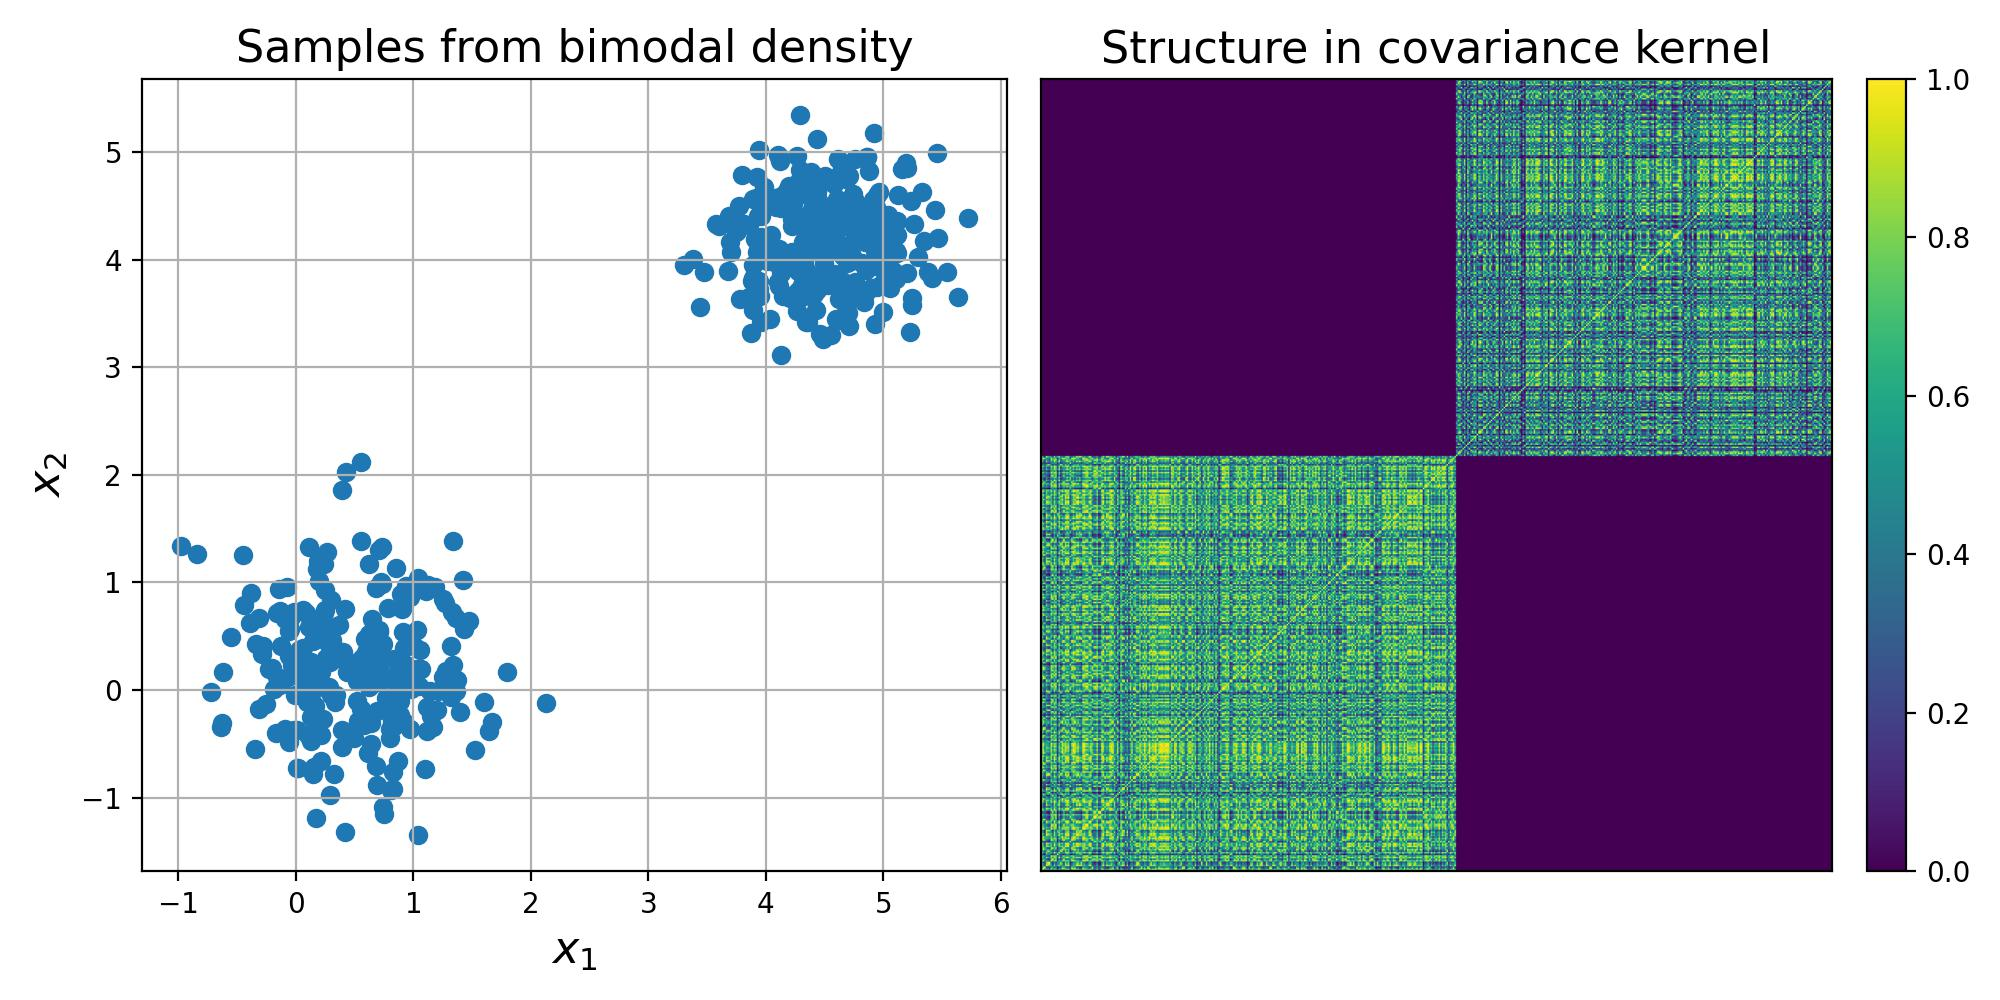
\includegraphics[width=0.75\linewidth]{figures/structure_cov_kernel.jpg}
    \caption{Covariance kernel with block diagonal structure corresponding to particles sampled from a bimodal target density}
    \label{fig:cov_structure}
\end{figure}

 % This will be done through a multi-fidelity setup, leveraging Approximate Control Variates (ACVs) in particular for efficient representation of the confining force.

Next, we provide background on multi-fidelity estimation using ACV estimators, before reviewing work leveraging multiple models for SVGD.


% \subsection{Gradient-based MCMC Methods}

% SVGD differs from conventional gradient-based MCMC methods in its evolution of a co-ordinated particle ensemble instead of simulation of Markov chains with individual particles. In particular, the Euler-discretized Langevin dynamics simulates a Markov chain with the rule:

% \begin{equation}
%     x_{i+1} \leftarrow x_i + \frac{\epsilon}{2}\nabla \log p(x_i) + \epsilon \eta_i
% \end{equation}

% where $\eta_i \sim \CN(0, \epsilon)$ injects Gaussian noise at each step to prevent collapse to the MAP solution. 
% For Bayesian inference, Stochastic Gradient Langevin Dynamics (SGLD) \citep{welling_bayesian_2011,brosse_promises_2018} permits use of large-scale datasets through unbiased gradient estimators based on small mini-batches of the data, potentially augmented with control-variates for variance reduction. 
% While these approaches to Langevin dynamics are extremely relevant to discussions of variance reduction techniques for MCMC methods, the key ideas do not translate directly to the SVGD setting: instead of distributing workload amongst an ensemble of particles, these reduce the costs of likelihood evaluation conditioned on a particular realization of parameters $x$.


\subsection{Approximate Control Variates for Multi-fidelity Estimation}\label{ss: acv}

% \textcolor{red}{Stealing the text from acv with uq with some cuts}

Consider a mapping $Q=f_0(Z)$ that relates the random vector $Z \in \mathbb{R}^{n_{z}}$ and the random variable $Q \in \mathbb{R}$. The expected value of $Q$ is often approximated by a standard $N$-sample Monte Carlo (MC) estimator:
\begin{align}\label{eqn:mc}
    \mathbb{E}\left[Q_0\right] 
    \approx \hat{Q}_0 := \frac{1}{N} \sum^{N}_{j=1}f_0(z^{(j)}),
\end{align}

where $z^{(j)} \sim p(Z)$ are independent and identically distributed (i.i.d.) samples drawn from the probability distribution of $Z$. The MC estimator $\hat{Q}$ is unbiased, making its estimator error contributed entirely by its variance $N^{-1}\Var[Q]$. When using computationally intensive models, the number of samples $N$ that can be afforded may not be sufficiently high to limit this variance.

To reduce the estimator variance, multi-fidelity methods leverage an ensemble of low-fidelity models whose outputs are correlated with the high-fidelity model of interest but with diminished costs. 

Control variates (CVs) are a widely used classical method for variance reduction in Monte-Carlo methods. 
The general approach is to identify another function $f_1$, such that the traditional expected value estimator described in Equation~\ref{eqn:mc} can be replaced by one constructed with $f_0 - f_1$, with smaller variance. The function $f_1$ is then referred to as a control variate. 
Typically, selection of $f_1$ (generalized to selection of $\{f_i\}, i=1, \cdots, M$) and identifying a rich set of candidate CVs is a non-trivial procedure barring the exceptions where CVs can be identified from domain knowledge. 
Linear transformations of the score function have been one of the popular choices given the high canonical correlations with the target that result in better variance reduction, and their straightforward incorporation into modern MCMC methods with gradient information and marginalization of hyperparameters \citep{papamarkou_zero_2014,oates_control_2017}. \cite{si_scalable_2021} extends CV identification to the high-dimensional settings by proposing a variational formulation based on Stein operators.
% \footnote{\textcolor{red}{Technically these are control functionals rather than control variates? \citep{oates_control_2017}}}.


In the context of multifidelity methods however, we typically already have access to a hierarchy of models, where each available low-fidelity model can be leveraged as a control variate, but their respective expectations must be computed from samples too. The approximate control variate (ACV) technique \cite{Gorodetsky2020, bomarito_optimization_2022} provides a rigorous formulation for deriving reduced-variance estimators in this setting.
This method introduces $M$ auxiliary random variables $Q_{m}$ for $m=1,\ldots,M$ that are outputs of the corresponding (e.g., low-fidelity) models $Q_{m} =f_{m}(Z)$, then combines the corresponding MC estimates of each low-fidelity model, $\hat{Q}_{m}$, into a single estimator. The ACV estimator, which we denote $\tilde{Q}$, can be written as:
\begin{align}
        \Tilde{Q}(z,\alpha,\CA) &:= 
        \hat{Q}_{0}(z_{0})+\sum^{M}_{m=1}\alpha_{m}\left( \hat{Q}_{m}(z^{\ast}_{m})-\hat{\mu}_{m}(z_{m}) \right) \nonumber\\ 
        &= \hat{Q}_{0}(z_{0})+\sum^{M}_{m=1}\alpha_{m}\left( \hat{Q}_{m}(z^{\ast}_{m})-\hat{Q}_{m}(z_{m}) \right),     \label{eqn:ACV-Formula}
\end{align}
where $\hat{\mu}_{m}$ is an MC estimate for the $m$th model mean, $\alpha = \left[ \alpha_{1}, \ldots, \alpha_M \right]$ is a vector of control variate weights, and the input samples $z$ are partitioned into subsets $z_{0}$, $z_{m}$, and  $z^{\ast}_{m}$ according to a sample partitioning strategy $\CA$. The control variate weights $\alpha$ and the sample partitioning strategy $\CA$ are hyperparameters of the estimator.
%that are chosen to optimally reduce the estimator variance. 

Since the ACV estimator is unbiased with respect to the high-fidelity model, its error is equal to the estimator variance. To express this variance mathematically, we introduce a vectorized notation for the ACV estimator:
\begin{align}\label{eqn:vectorized-acv}
    \Tilde{Q}(z;\alpha,\CA) = \hat{Q}_{0} + \alpha^{\top}\Delta,
\end{align}
where $\Delta:=\left[ \Delta_{1}(z_{1}^{\ast},z_{1}), \ldots,  \Delta_{M}(z_{M}^{\ast},z_{M})\right]$, $\Delta_{m}(z_{m}^{\ast},z_{m}):=\hat{Q}_{m}(z^{\ast}_{m})-\hat{Q}_{m}(z_{m})$, and the explicit dependence on the inputs $z_{m}$ and $z_{m}^{\ast}$ are omitted for simplicity of notation. The ACV estimator variance is then:
\begin{align}\label{eqn:acv-variance}
    \Var[\Tilde{Q}(z;\alpha,\CA)] = \Var[\hat{Q}_{0}] - \alpha^{\top}(\Cov[\Delta, \Delta])^{-1}\alpha + 2 \alpha^{\top} \Cov[\Delta, \hat{Q}_{0}].
\end{align}
The estimator variance is dependent on the covariances between each model output, the control variate weights, and the sample partitioning that influences how each $\Delta$ term covaries with each other and with $\hat{Q}_{0}$. If the exact covariance between each model output is known, then the optimal weights for a given ACV sample allocation $\CA$ can be computed by minimizing \eqref{eqn:acv-variance}. The optimal weights are:
\begin{align}\label{eqn:alpha-star-acv}
    \alpha^{\ast}(\CA)=-\Cov[\Delta, \Delta]^{-1}\Cov[\Delta, \hat{Q}_{0}],
\end{align}
and when these weights are set to their optimal values, the ACV estimator variance is~\cite{Gorodetsky2020}:
\begin{align}\label{eqn:acv-variance-opt}
    \Var[\Tilde{Q}^{\alpha^{\ast}}](\CA) = \Var[\hat{Q}_{0}] - \Cov[\Delta, \hat{Q}_{0}]^{\top} \Cov[\Delta, \Delta]^{-1}\Cov[\Delta, \hat{Q}_{0}].
\end{align}

The sample partitioning $\CA$ determines how much computational workload is distributed to each model. The well-known multi-fidelity Monte Carlo (MFMC) \cite{peherstorfer_optimal_2016} and multi-level Monte Carlo (MLMC) \cite{giles_multilevel_2015} methods can be shown to be special cases of ACV that differ in the family of possible $\CA$ choices. Solving for the optimal sample partitioning strategy $\CA^{\ast}$ is more intensive than solving for the optimal weights $\alpha^{\ast}$ but many tools \cite{bomarito_multi_2020, jakeman_pyapprox_2023} are available to approximately solve the optimization problem:
\begin{align}
    \min_{\mathcal{A}\in\mathbb{A}} &\quad \Var[\tilde{Q}(Z;\alpha^{\ast},\mathcal{A})] \label{eqn:mxmcpy}\\
    \text{subject to} &\quad \mathcal{W}(w,\mathcal{A})\leq w_{\text{budget}},\label{eqn:mxmcpy_constraint}
\end{align}
where $\mathbb{A}$ is a wide set of predefined allowable set of sample allocations, $w_{\text{budget}}$ is the total budget constraint, and $\mathcal{W}(w,\mathcal{A})$ computes the total cost of the estimator under model costs $w := [w_0, \ldots, w_M]$ and sample allocation $\CA$.

Importantly, the solutions to \eqref{eqn:mxmcpy} and \eqref{eqn:alpha-star-acv} are only computable with knowledge of the model output covariance matrix, $\Sigma = \Cov\left[ f_0(Z),\ldots,f_M(Z)
\right]$, as well as the model costs vector $w$. 

Alternative sampling-based estimators beyond the ACV formulation above, such as the multilevel best linear unbiased (MLBLUE) estimator from \cite{schaden_multilevel_2020} 
can produce impressive variance reduction like ACV. 
In fact, the generalized linear grouped ACV estimator (GACV) \cite{gorodetsky_grouped_2024} generalizes these methods. Though exact parametrizations may differ across estimators, they share common features of estimator weights and sample allocations.

\subsection{Related Work: Multi-level SVGD}

In this section, we highlight two previous approaches that leverage estimation with multiple models to drive the SVGD updates and achieve significant cost reduction in the process. 

While these are important efforts that provably result in more efficient SVGD-based approximations, we point out key limitations that restrict broader adoption:

\begin{enumerate}
    \item The multilevel approach is limited to model ensembles with constraints on the cost-accuracy relationships. For instance, both methods above rely on coarser discretizations of the forward operator. They cannot operate with more general ensembles that commonly arise in scientific development, including reduced-order models and surrogates.

    \item Effectiveness of not blending? 
\end{enumerate}

In addition to the direct combination of particle position updates driven by different fidelities, our work also introduces a novel approach to inform covariance estimation on the fly.



\section{Methodology}



% \subsection{Baseline: Bifidelity SVGD}
% Before we propose the multi-fidelity ACV construction, it is is still instructive to demonstrate the basic idea of partitioning the likelihood evaluation costs through a bifidelity surrogate SVGD construction, where a subset of particles evaluated under the lower-fidelity target density are `corrected' through the corresponding high-fidelity density gradient update.

% Let $n_0$ be the number of particles that are updated under both high and low-fidelity likelihood models. Let $n_1$ represent the number of particles updated only under the low-fidelity representation.

% Then the new updates take the form:
% \begin{align}
%     x_i^{l + 1} &\leftarrow x_i^l + \epsilon_l\hat{\phi}^{\ast}_{\text{BF}}(x_i^l)
%     \label{eq: bf_svgd_basic}
% \end{align}

% where:
% \begin{align}
%     \hat{\phi}^{\ast}_{\text{BF}}(x) &= \frac{1}{n_1}\left[\sum_{j=1}^{n_1} k(x_j^l, x) \nabla_{x_j^l}\log p_1(x_j^l) + \nabla_{x_j^l}k(x_j^l, x)\right]
%     + \frac{1}{n_0}\left[\sum_{j=1}^{n_0} k(x_j^l, x) \nabla_{x_j^l}\log \left(\frac{p_0(x_j^l)}{p_1(x_j^l)}\right)\right]
%     \label{eq:bf_gradient_expr}
% \end{align}

% The key features of the update are:

% \begin{enumerate}
%     \item The correction term does not contain a repulsive force term, and the repulsion term in the first half of the equation has to accomodate particles updated under a single as well as multiple fidelities.

%     \item The magnitudes of the score difference are smeared over the domain through the correlations between the high-fidelity and the remainder of the low-fidelity particles. 

%     \item The subset of particles used to define the correction term is \emph{randomized} from iteration to iteration. This is key to all particle positions eventually correcting to fit the target high-fidelity density.
% \end{enumerate}

% % While we do not draw directly from the theory of numerical methods and ODE integrators


% % The additive correction is learnt subsets that are randomized from iteration to iteration. In this case, the repulsion term is driven by particle positions under the misspecified likelihood during the initial step and a mixture of particles driven by multiple fidelities in subsequent steps.

% A quality measure is needed to determine when a sequence of samples is converging or not to the target density in SVGD. Stein's method provides a tool to define a discrepancy measure between densities $p$ and $q$ that can measure asymptotic bias in approximate MCMC samplers \cite{gorham_measuring_2017} and is also tailored to SVGD-based inference.\footnote{A key benefit is the ability to evaluate the discrepancy without explicit density estimation of $q$ for the propagated particles, unlike the more popular KL-divergence.} For smooth functions $f(x) \in \CF$, the Stein discrepancy measure\citep{liu_kernelized_2016} is defined as :

% \begin{equation}
%     \mathbb{S}(q, p) = \max_{f \in \CF}\left(\EE_q[\nabla_x \log p(x)f(x) + \nabla_x f(x)]\right)^2 \label{eq:ksd_regular}
% \end{equation}

% \cite{liu_kernelized_2016} define a computationally tractable version of this by assuming $\CF$ to be a ball in a reproducing kernel Hilbert space (RKHS) associated with a smooth positive definite kernel $k(x, x')$. Denoting $\nabla_x \log p(x)$ by $s_p$, the Kernelized Stein Discrepancy (KSD),

% \begin{align}
%     \mathbb{S}(q, p) &= \mathbb{E}_{x, x' \sim q}[u_p(x, x')] \nonumber \\ 
%     &= \mathbb{E}_{x, x' \sim q}[s_p(x)^{\top} k(x, x')s_p(x') + s_p(x)^{\top} \nabla_{x'}k(x, x') + \nonumber\\ 
%     & \nabla_x k(x, x')^{\top}s_p(x') + \operatorname{trace}(\nabla_{x, x'}k(x, x'))] \label{eq:ksd_kernel}
% \end{align}

% is the empirical evaluation of $\mathbb{S}(q, p)$, which can be estimated through the following $U$-statistic:

% \begin{align}
%     \hat{\mathbb{S}}_u(q, p) = \frac{1}{n(n-1)}\sum_{1 \leq i \neq j \leq n} u_p(x_i, x_j)
% \end{align}

% % We assess the performance of each SVGD variant through the Kernelized Stein Discrepancy (KSD), which represents the maximum violation of Stein's identity when the expectation is computed under $q$ instead of $p$ and therefore avoids explicit integration under the target. 

% Theory for the weak convergence of KSD is developed in \cite{gorham_measuring_2017}, and suggests that commonly used KSD formulations fail to detect non-convergence for violating sample sequences, even for simple Gaussian targets in small to modest dimensions ($d \geq 3$). 
% In examples showcasing SVGD, we use the Inverse Multiquadric (IMQ) Kernel i.e. $k(x, x') = (c^2 + ||x - x'||_2^2)^\beta$ in the KSD estimator, in line with their recommendations, with $\beta=-1/2$ and $c=1$. A comparison of the IMQ and RBF kernel basis functions is shown in Figure~\ref{fig:imq_vs_rbf}, with the RBF kernel defined as $k(x, x') = \exp(-||x - x'||_2^2 / h^2)$.

% Our initial demonstrations do not specify an explicit prior and likelihood but instead evaluate the effectiveness of the proposed estimator on an ensemble of closed-form target density functions. Figure~\ref{fig:svgd_sf_vs_bf_surrogate_rbf} shows an example of mapping from an initial set of particles to a Gaussian mixture high-fidelity target density, while leveraging a lower-fidelity density $p_1$ which corresponds to one of the modes.
% \begin{align}
%     p_1(\mathbf{x}) &= \CN\left(\mathbf{x}; \begin{bmatrix}-2.5 \\ -1.5\end{bmatrix}, \begin{bmatrix}1.5 & 0 \\ 0 & 0.5\end{bmatrix}\right)\\ \nonumber
%     p_2(\mathbf{x}) &= \CN \left(\mathbf{x}; \begin{bmatrix}0.5 \\ 0.2\end{bmatrix}, \begin{bmatrix}2.0 & 0.3 \\ 0.3 & 0.5\end{bmatrix}\right)\\ 
%     p_0(\mathbf{x}) &= \sum_{j=1}^2 \pi_j \CN(\mathbf{x}; \mu_j, \sigma_j) \quad, \pi_1 = \pi_2 = 0.5 \nonumber
%     \label{eq:p0p1_toy_example}
% \end{align}

% \begin{figure}[htbp]
%     \centering
%     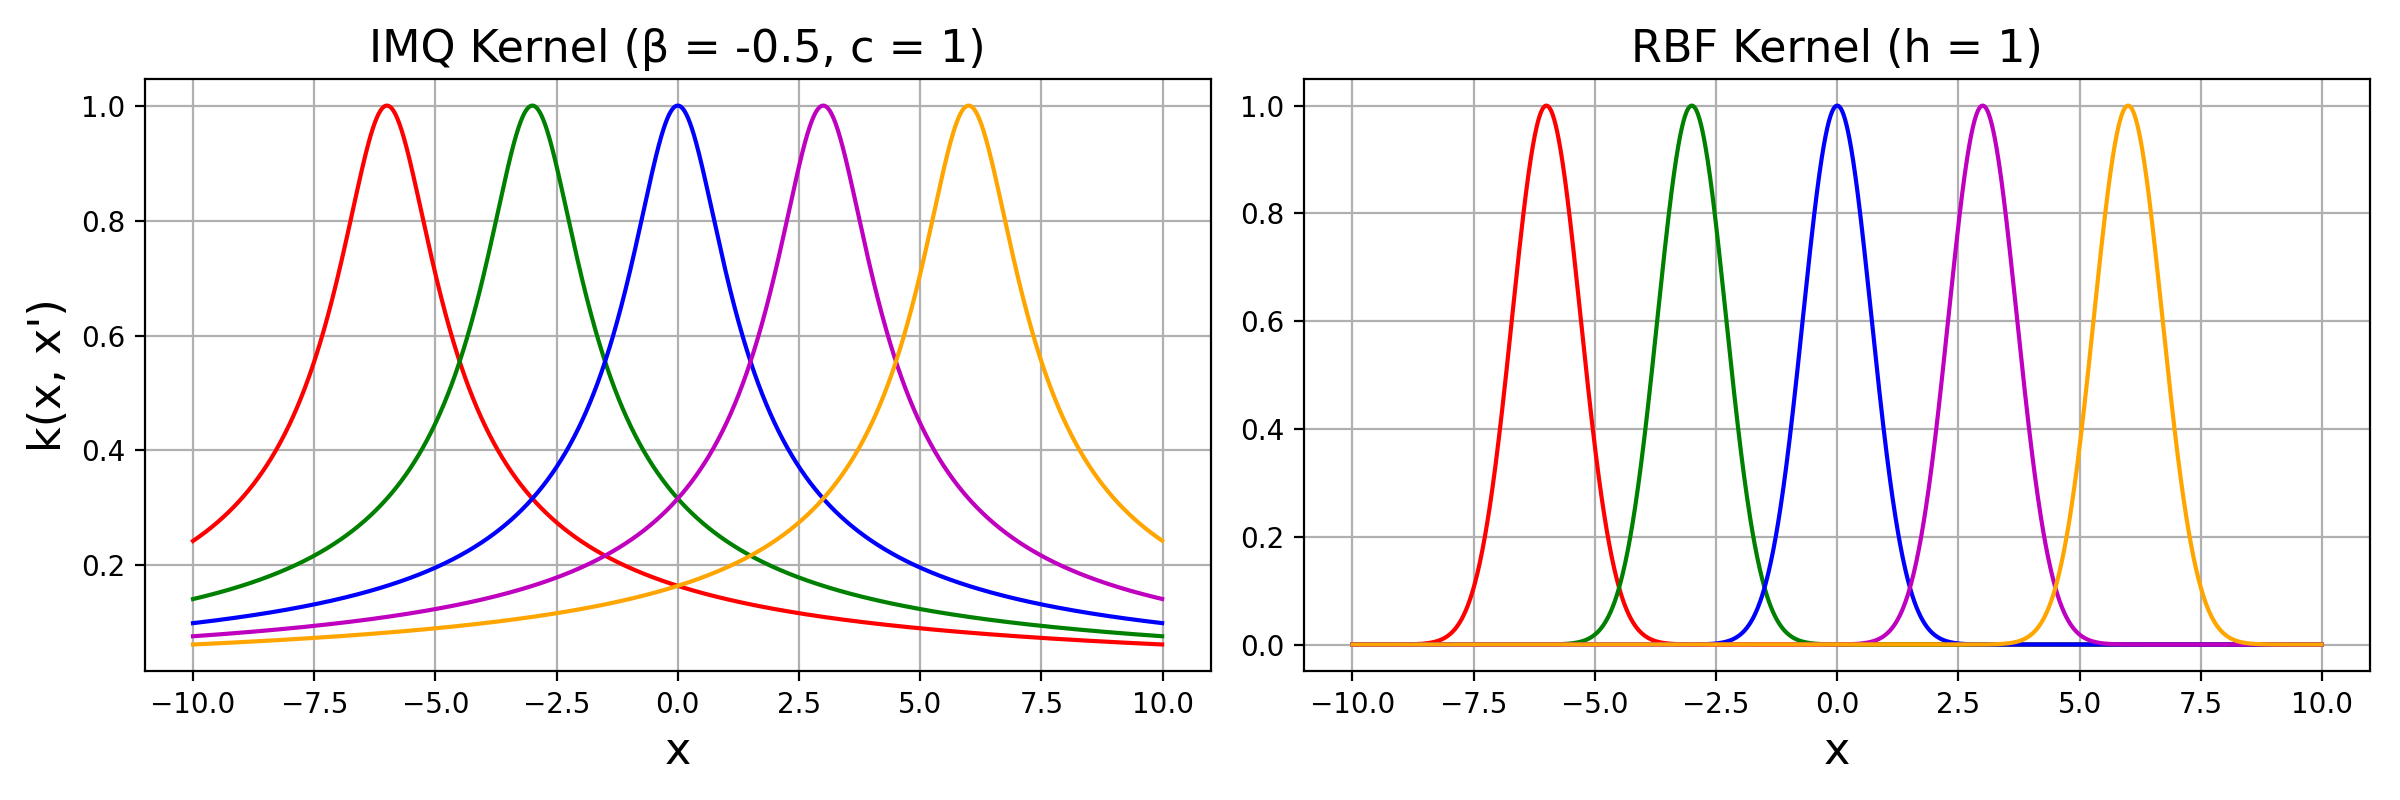
\includegraphics[width=0.85\linewidth]{figures/imq_vs_rbf_basis_functions.png}
%     \caption{Examples of basis functions generated through IMQ and RBF kernels for $d=1$. The most significant difference is the smoothly decaying tails for RBF, which falls in the class of KSDs that may fail to detect non-convergence.}
%     \label{fig:imq_vs_rbf}
% \end{figure}


% \begin{figure}[htbp]
%     \centering
%     % 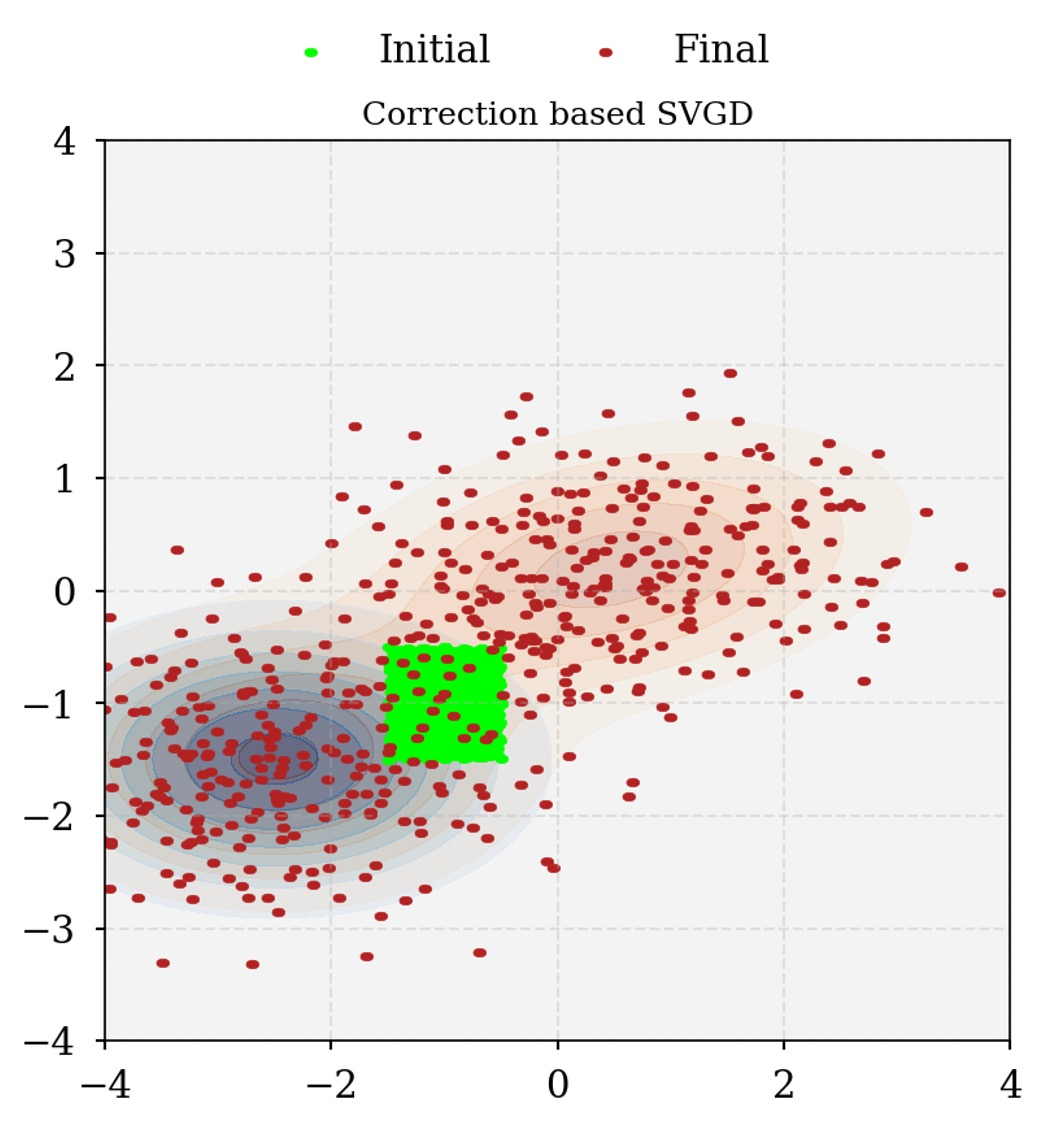
\includegraphics[width=0.75\linewidth]{figures/svgd_scalable_mixture_hf.jpg}
%     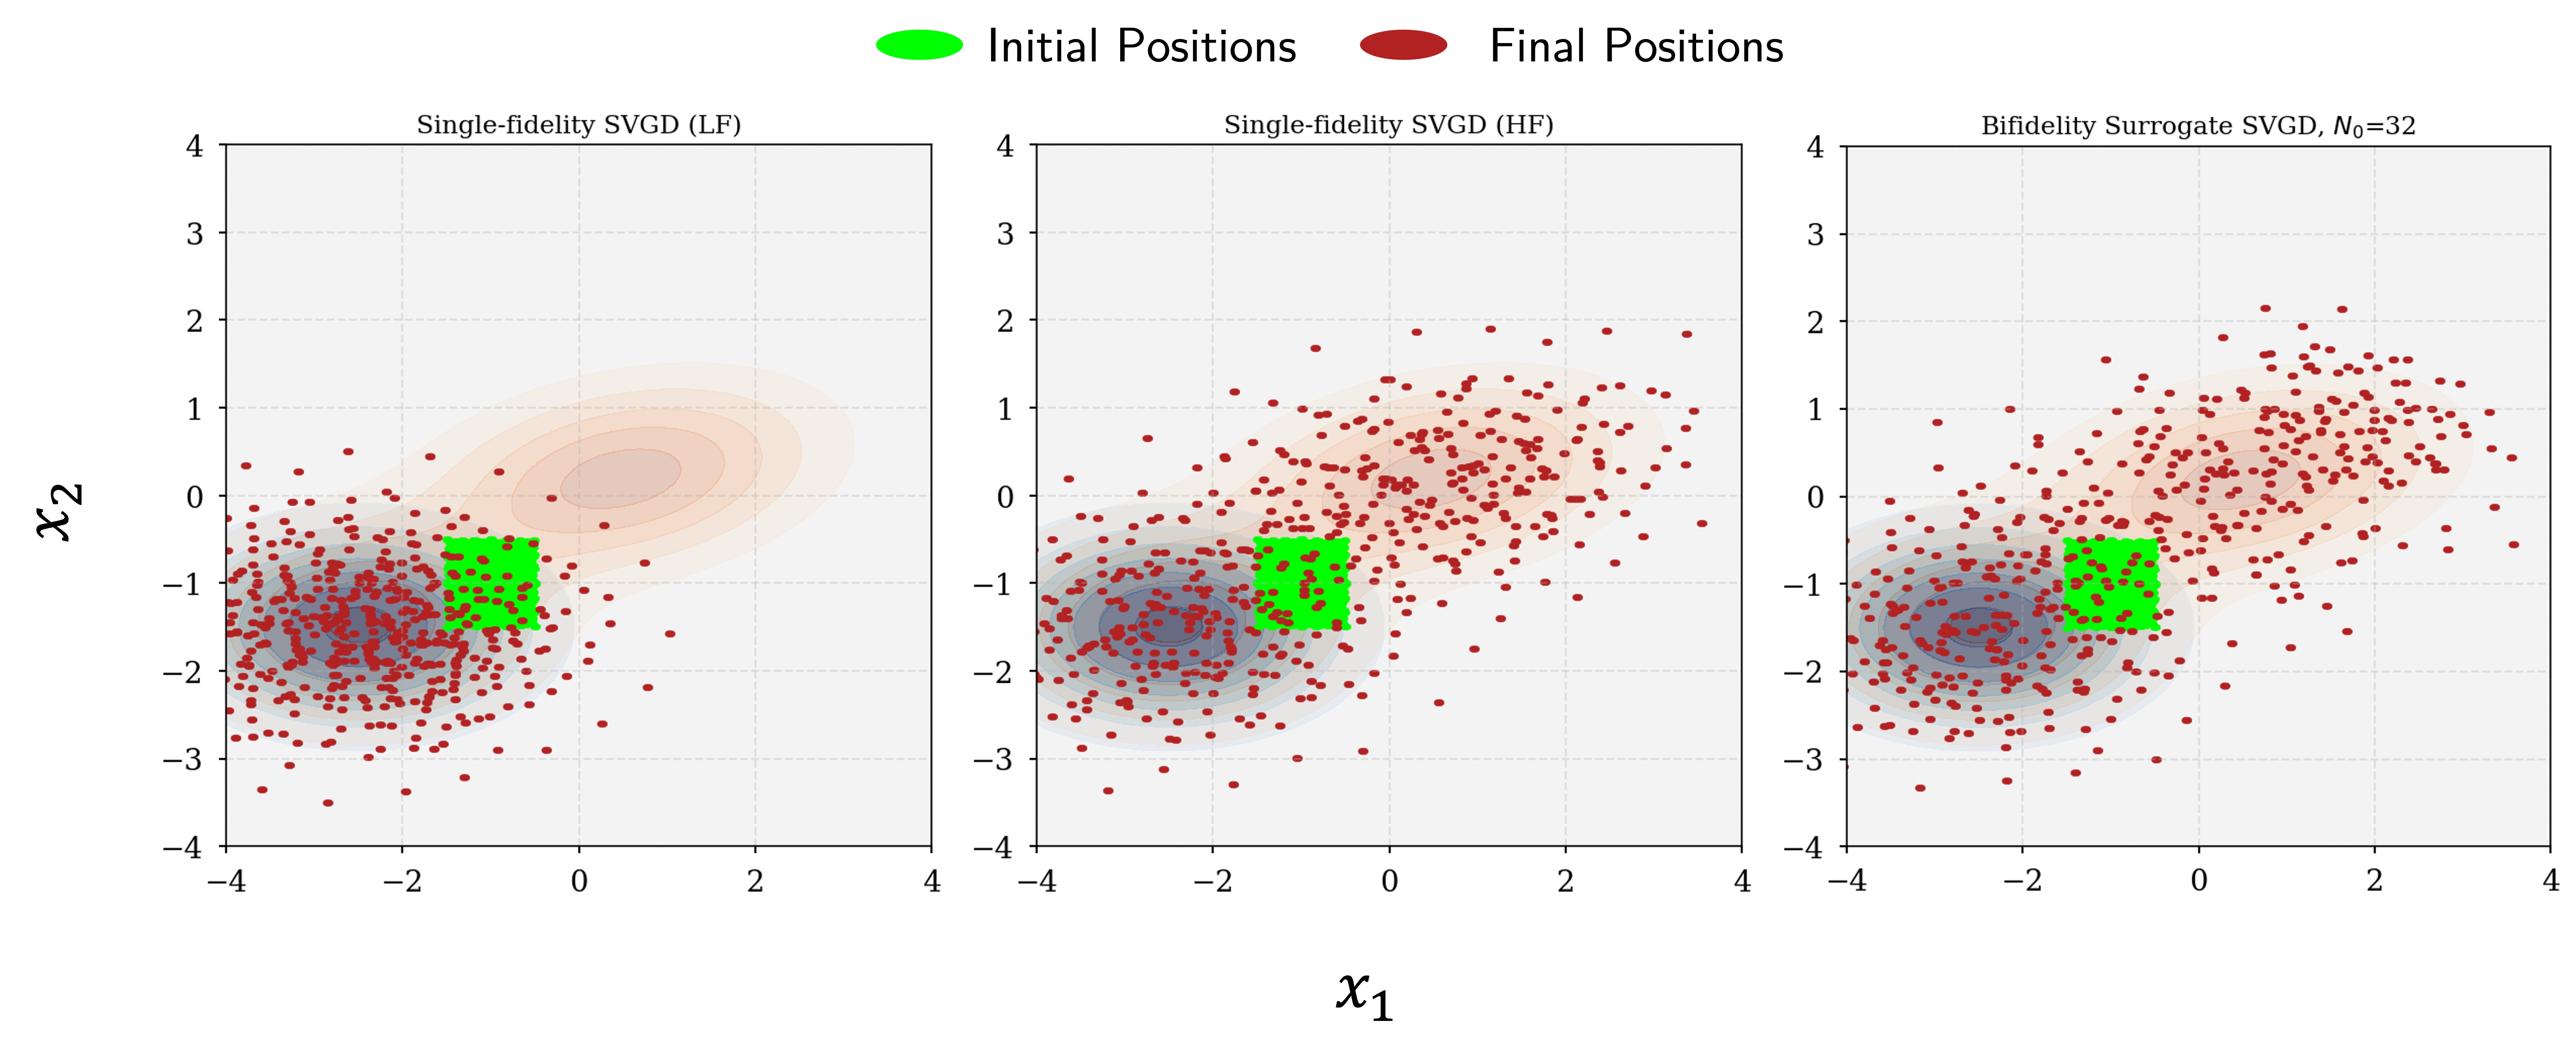
\includegraphics[width=\textwidth]{figures/bifidelity_svgd_comparisons_gaussian_mixture_rbf.jpg}
%     \caption{Particles mapping to the high-fidelity target posterior based on the surrogate bifidelity gradient estimator for SVGD (right) and the single fidelity estimators under individual LF and HF targets (left and middle). The contours of the high-fidelity distribution, a Gaussian mixture, are marked in orange, while those of the unimodal lower-fidelity target are marked in blue. The particle positions at the initial timestep, drawn through quasi-MC uniform sampling, are marked in green, and those in brown represent the positions at the final timestep. 32 particles are used to correct the low-fidelity estimate at each step for the surrogate estimator.}
%     \label{fig:svgd_sf_vs_bf_surrogate_rbf}
% \end{figure}

% Next, KSD is reported for target ensembles with total number of particles set to \textnormal{\{16, 32, 64, 128, 256, 512\}}
% to measure the gap between the density induced by SVGD particles at the final update step and samples from the true posterior. We compare KSD trends for vanilla SVGD and the bifidelity-surrogate SVGD (BFS-SVGD), the latter with a varying number of particles used for the correction term.





% % To better interpret the efficacy of the bifidelity update, we first visualize the evolution of the contributors to the velocity field i.e. SVGD gradient at different time steps.

\subsection{Generalized Multifidelity-SVGD (MF-SVGD)}

The multi-fidelity update for SVGD partitions the gradient, which is typically estimated through the standard MC estimator, in the style of ACVs so that particles are apportioned to target densities of different fidelities at every iteration. 
% The key differences compared to the surrogate SVGD estimator we discussed in the previous section would stem from both the unbiasedness of the ACV estimator and the ability to accomodate arbitrary model ensembles with error-optimal particle allocations.

To ensure consistency with the notation introduced in subsection~\ref{ss: acv}, we set $z_i^l \triangleq \mathbf{x}^{(l)} \setminus x_i^l$ for a particle ensemble $\mathbf{x}^{(l)}$ at iteration $l$. Next, by linearity of expectation, we partition the overall gradient $\hat{\phi}^{\ast}$, and replace the confining force by its ACV representation. The repulsive force computation, which depends only on pairs of particles, is not affected by the choice of model, and therefore does not admit a control-variate based representation -- the SVGD update for the individual models / densities features \emph{identical} contributions from the repulsive force.  Using $\Psi$ as shorthand to denote any appearance of CF, we can 
\begin{align}
        \tilde{\psi}(x_i^l, z_i^l, \alpha, \CA) = \tilde{\psi_0}(x_i^l, z_0) + \sum_{m=1}^M \alpha_m \left(\hat{\psi}_m(x_i^l, z_m^{\ast}) - \hat{\gamma}_m(x_i^l, z_m)\right),
        \label{eq: cf_update}
\end{align}
followed by:
\begin{align}
    x_i^{l + 1} \leftarrow x_i^l + \epsilon_l\tilde{\psi}(x_i^l, z_i^l, \alpha, \CA) + \epsilon_l\left[\frac{1}{n}\sum_{j=1}^{n} \nabla_{(z_j^l, x_i^l)} k\left((z_j^l, x_i^l), x\right)\right],
    \label{eq: mf_svgd_proposal_1}
\end{align}
where $\tilde{\psi}_{(\cdot)}$ is shorthand for $\left[\frac{1}{n_{(\cdot)}} \sum_{j=1}^{n_{(\cdot)}}k\left((z_j^l, x_i^l), \cdot\right) \nabla_{(z_j^l, x_i^l)} \log p_{(\cdot)} \left((z_j^l, x_i^l)\right)\right]$, and $n_i$ denotes the fraction of particles out of $n$ particles used in the score computation for model $i$.

Other representations of the gradient estimator may also focus on reducing the computational cost of computing pairwise interactions apart from the score computation. We leave investigation of these choices to future work and discuss the ACV-based formulation in greater detail as a first step towards a flexible multi-fidelity version of SVGD.

\subsection{Pilot Sampling for Covariance Estimation}

\subsection{Overall MF-SVGD Algorithm}

% \subsubsection{Offline Pilot Sampling}

% As the particles initialized with density $q_0$ are propagated towards the target $p_i$, the ACV estimates need to be recomputed for every intermediate density $q_i$, ideally with a smaller subset of particles that can establish a fairly accurate estimate of the pilot covariance matrix. 

% A method for offline pilot sampling is presented below. It relies on generating particles sequences under some choice of $p_i$ and number of pilot particles $N_p$. Then, keeping this sequence fixed, we recover the particle-wise weighted score function values at every step for all model fidelities. Finally, we summarize the particle-wise correlations based on the score function values to establish a fixed stepwise sample allocation. 

% We use the simplest variation of ACV for our ACV-SVGD based framework that computes multi-fidelity estimates for a single output / scalar QoI. This implies that for a $d$-dimensional target posterior, the sample allocations for each update directions are computed separately based on optimal variance reduction in the respective components of the gradient / velocity field. While this is by far the most scalable approach, there is also potential to exploit the correlations between gradient components for even greater variance reduction \citep{dixon_covariance_2024}. 




% % The simplest method considers non-adaptivity of learning rates and correlations established through pilot sampling.

% % \begin{algorithm}[ht!]
% % \caption{Non-adaptive Pilot Sampling-based MF-SVGD}\label{alg:pilot_sampling_termination}
% % \begin{algorithmic}[1]
% % \item Pilot sampling loop - either: take a small set of particles propagated across all fidelities, and get the correlations from these. OR: we choose a specific fidelity, and obtain all the intermediate gradients. Then the question is: keeping these positions fixed, what are the operator action correlations for the remaining fidelities? 
% % % \textcolor{red}{check! do these perform the same computation?}

% % \item given stagewise correlations, determine particle allocations, compute respective updates and form ACV estimator.
% % \end{algorithmic}
% % \end{algorithm}

% \begin{algorithm}[H]
%   \caption{Offline Pilot Sampling}\label{alg: pilot_sampling_non_adaptive}
%   \begin{algorithmic}[1]   
%   \State \textbf{Input:} Step size $\epsilon$, densities $p_i(x)$ for $i=0,\dots,M-1$, kernel $k(x,x')$, initial particles $\{x_j^{(0)}\}_{j=1}^{N_p}$, total budget $B$.
%   \State \textbf{Output:} Covariance matrix and sample allocations for $L$ iterations
%   \State Choose fidelity $i$ to compute deterministic particle sequences for $L$ iterations with step size $\epsilon$, obtain sequence $S_x  = \{\mathbf{x}^{(0)}, \cdots, \mathbf{x}^{(L - 1)}\}$, where $\mathbf{x}^{(l)} = \{x_i^{(l)}\}_{i=1}^{N_p} \sim q^{(l)}$
%   \State Using $S_x$, store gradient contributions to each particle from neighbour particles for each target density in the model ensemble at every step: $\Psi^{(j)} = \begin{bmatrix}
%       k(x_1, x_1)\nabla_{x_1} \log p_j(x_1) & \cdots & k(x_{n_p}, x_1) \nabla _{x_{n_p}}\log_{x_{n_p}}p_j(x_{n_p}) \\
%       \vdots & \vdots & \vdots \\
%       k(x_1, x_{n_p})\nabla_{x_1} \log p_j(x_1) & \cdots & k(x_{n_p}, x_{n_p}) \nabla _{x_{n_p}}\log_{x_{n_p}}p_j(x_{n_p})
%   \end{bmatrix}$ and $\Psi = \{\Psi^{(j)}\}_{j=0}^{M-1}$
%   \State Obtain sample covariances $C_i^{(l)}$ for each particle using stored $\Psi^j$, and compute sequence of the mean covariance matrix $\{\hat{C}^{(l)}\}_{l=1}^{L}$ to set as ACV hyperparameters.
%   \State Obtain stepwise sample allocations and control variate weights: $\alpha^l, \CA^l \leftarrow \texttt{ACVEstimator}(B, \hat{C}^{(l)})$
% \end{algorithmic}
% \end{algorithm}

% An alternate approaches involves constructing a biased estimate of $\hat{C}^{(l)}$ by using gradients computed for all particles directly i.e. $K\nabla_{\mathbf{x}}\log p_i$. We illustrate these results in Figure~\ref{fig:svgd_gaussians_pilot_corrs} via an ensemble of Gaussian target densities, with $N_p=32$, $\epsilon=0.1$ and a synthetic cost vector $w=[1, 0.75, 0.25]$, from which the total budget is set to $B=64 \cdot \sum_i w_i$. The target $p_1$ is used to compute $S_x$.

% We show the log-densities of each of the ensemble members and the stepwise correlation estimates from the approach of Algorithm~\ref{alg: pilot_sampling_non_adaptive} as well as the alternate approximation, the former of which is more conservative in the correlation estimates.

% Our next steps will include testing various approaches to pilot sampling, including an online covariance estimation step, where a subset of propagated $N$ particles can be evaluated instead of an independent offline pilot set. 
% Finally, single-output and multiple output ACV estimators will be compared alongside the surrogate bifidelity estimator in various settings to establish the efficacy of the multi-fidelity framework. 

% \begin{figure}[htbp]
%     \centering
%     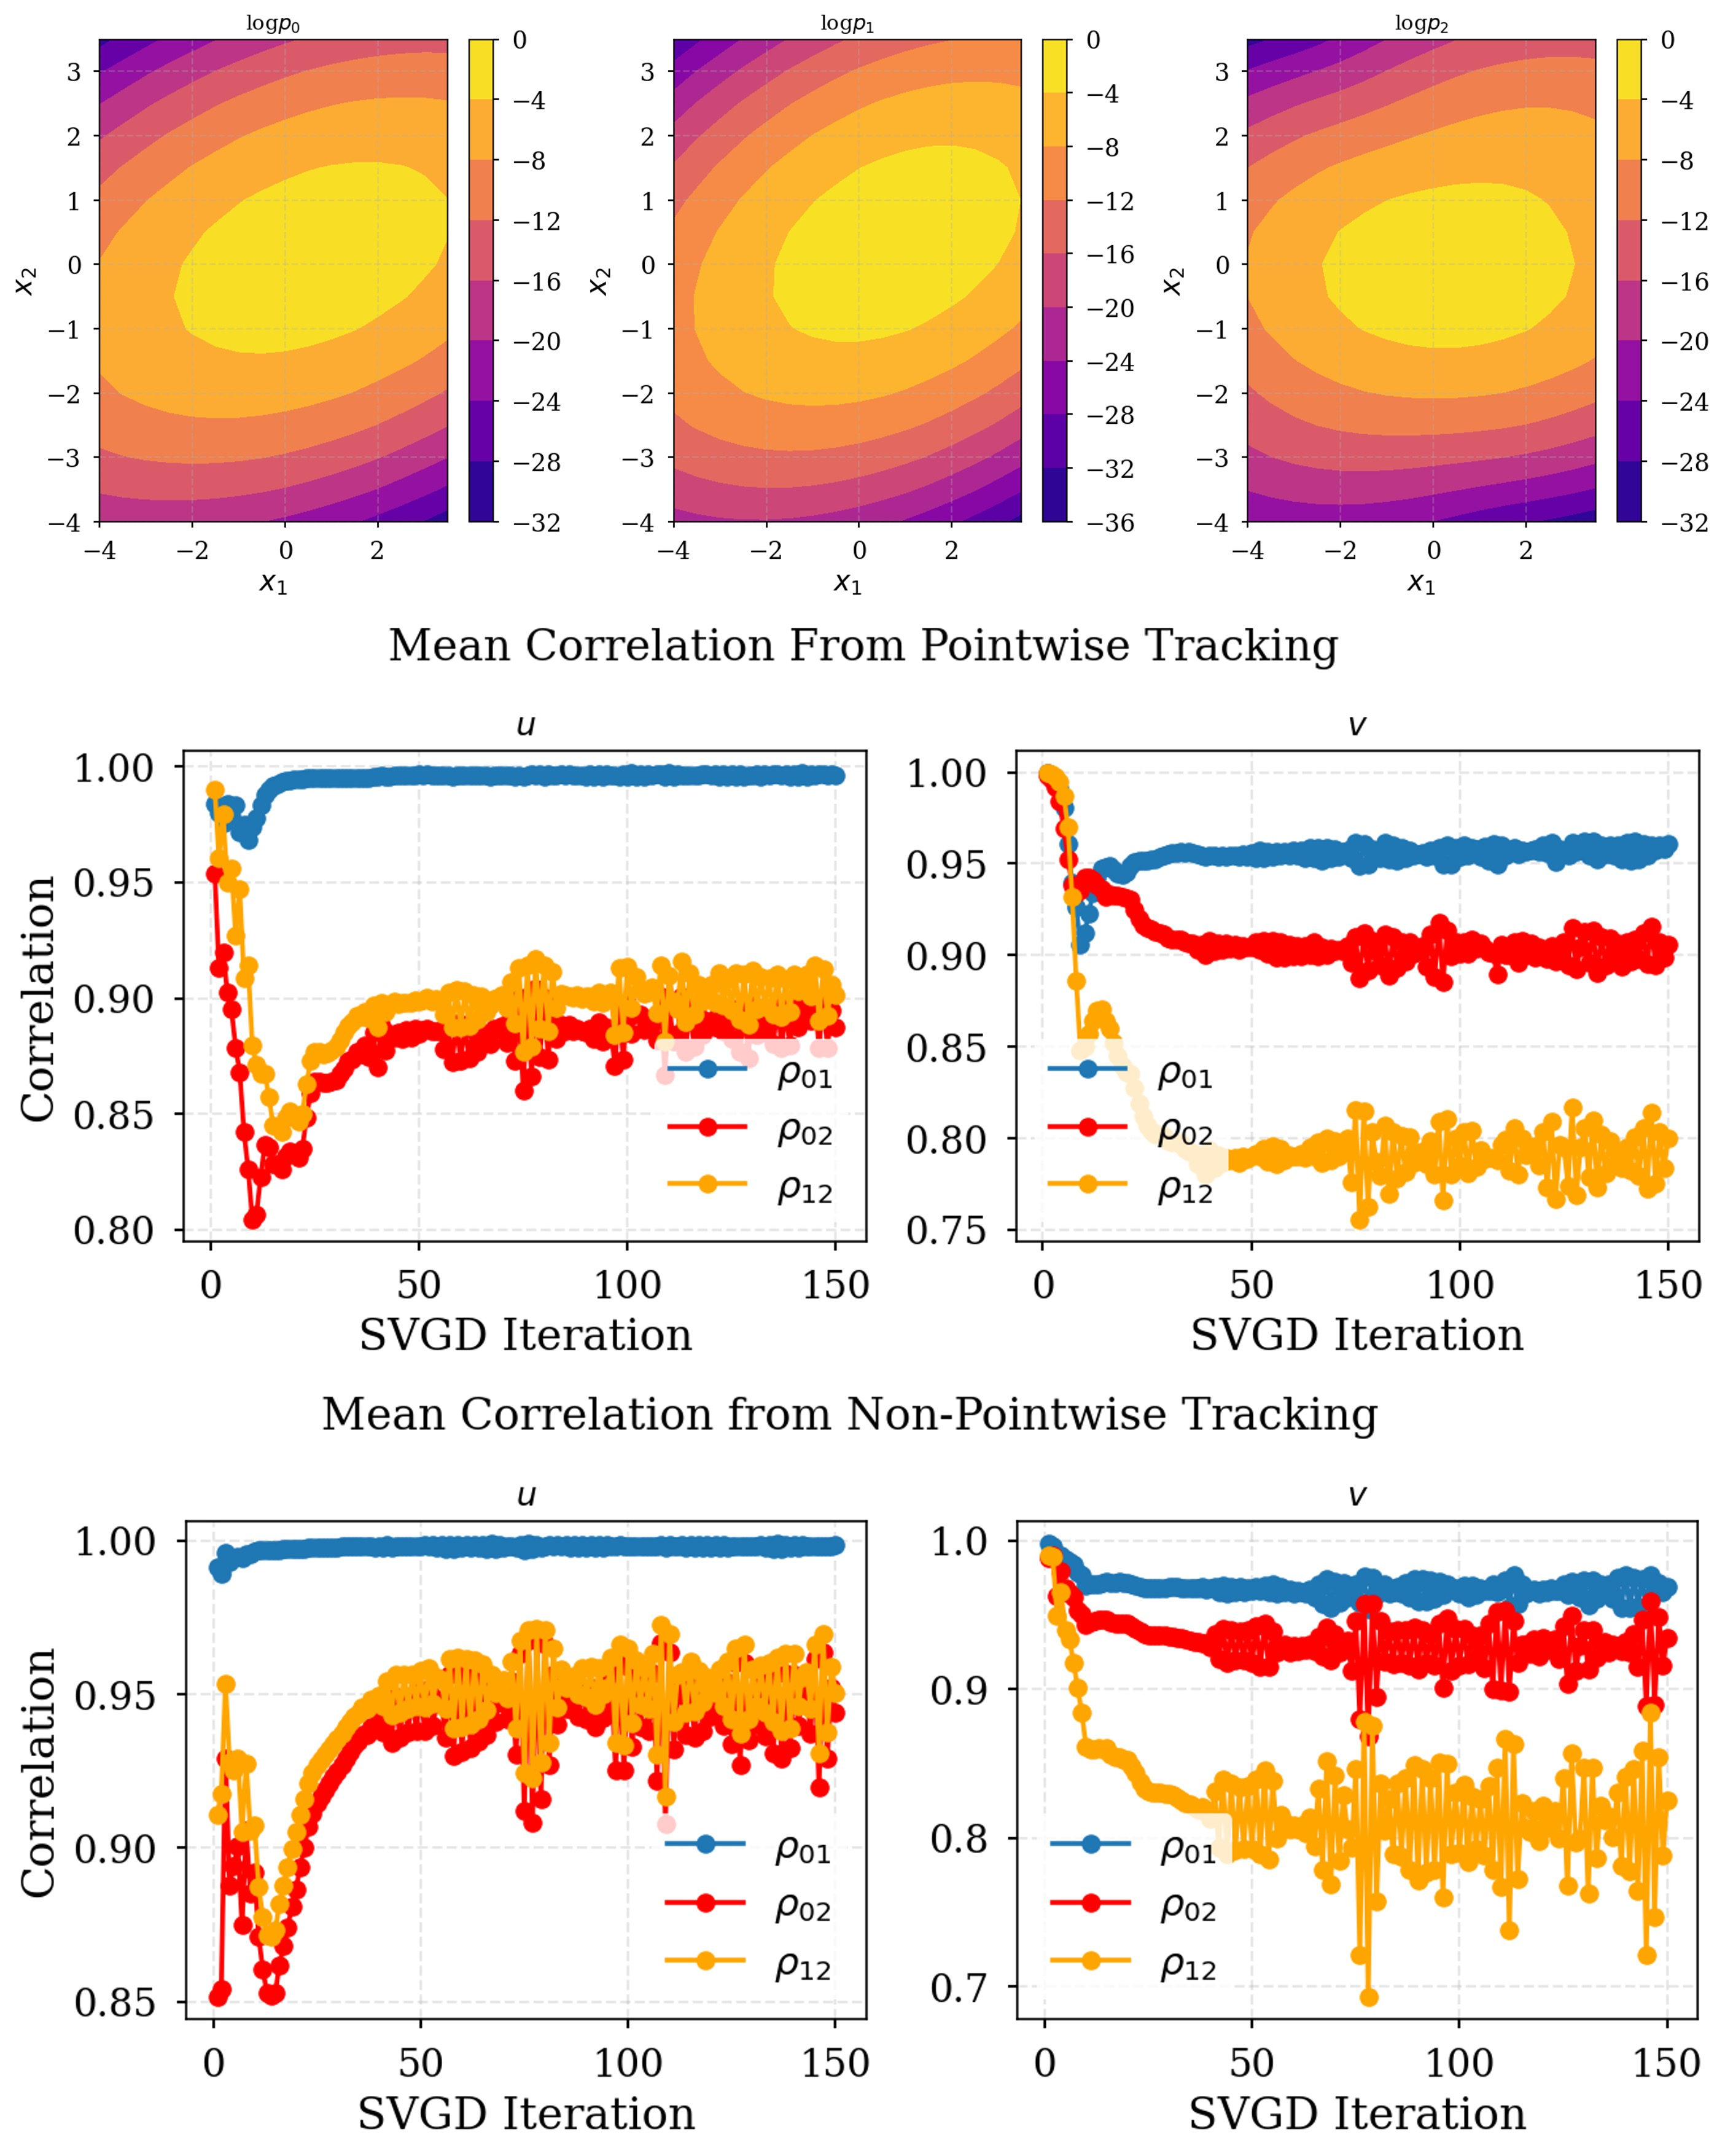
\includegraphics[width=0.8\linewidth]{figures/log_densities_corrs_composite.jpg}
%     \caption{Log-densities of each of the model ensemble members (top), followed by sample correlations calculated via \autoref{alg: pilot_sampling_non_adaptive} (middle) and the cumulative approximation for $N_p = 32$}
%     \label{fig:svgd_gaussians_pilot_corrs}
% \end{figure}

\section{Results}

\subsection{Multivariate Gaussian Model Problem}
To demonstrate the working of the algorithm, we use a simple benchmark problem where the target densities are multivariate Gaussians $\{p_i(x)\}_{i=0}^{M-1}$, with $M=3$, and each $p_i$ parametrized by its respective mean and covariance $(\mu_i, \Sigma_i)$:

The associated cost vector is given by $w=\{10^{-m}\}_{m=0}^{M-1}$.




\subsection{Estimator Performance for Monte-Carlo Integration}

\subsection{Bayesian Inference}
Given access to a model ensemble $f_i(x)$, $i=1, \cdots, M$ where the subscript indexes models from the highest to the lowest fidelity, and $x \in \RR^{n_x}$ is a random vector, the data-generating process and the log-likelihood functions corresponding to these outputs can be expressed as:
\begin{align}
 y_i = f_i(x) + \epsilon_i, \qquad L_i = \log p(\mathbf{y}_i | x) = \prod_{k=1}^N \log p(y_k | x)
 \label{eq: lik_fid_dgp}
\end{align}

where $\mathbf{y}_i = [y_1, \cdots, y_k, \cdots, y_N]$ are i.i.d. observations and $\epsilon_i$ is zero-mean additive noise.

Using the same prior density $p_o(x)$ in each of the inference setups for the individual models, the score function for the posterior PDF then simplifies to the following tractable expression that does not require evaluation of the normalizing constant:

\begin{align}
    \nabla_{x} \log p_i(x \mid D) = \nabla_x (L_i  + \log(p_o(x)),
    \label{eqn: bayes_rule_score}
\end{align}
% \subsection{Optimal Experimental Design via MF-SVGD Bayesian Inference}


% \subsection{Generalizing Compressed Representations to Higher Particle Counts}
% We consider the case where the original inference is performed on a small set of $N$ particles, but density estimation may be desired with additional particles at test time. 
% Then we need the ability to perform rapid approximation of positions for $K$ new particles introduced at test time. 
% This would require $\Mycomb[(N+K)]{2} - \Mycomb[N]{2} = \frac{1}{2}(K^2 + 2NK - K)$ additional distance calculations and $K$ potentially expensive likelihood computations followed by density estimation in the naive setting. 
% By contrast, a trained parametric simulator that 1. is `discretization invariant' in some sense by capturing the key relationships between existing particles 2. can allocate a large fraction of particles to one or more lower-fidelity models can rapidly convert these to high-quality posterior samples.

\section{Conclusions and Extensions}

In this work, we considered the application of multifidelity surrogate and multifidelity estimator techniques to a general-purpose non-parametric variational inference technique, namely Stein Variational Gradient Descent (SVGD). SVGD has numerous applications, including hypothesis testing, development of traditional CVs for MCMC, and  Bayesian inference for neural networks - settings with access to a smooth and differentiable posterior density. 

We proposed two alternate estimators that take advantage of lower-fidelity forward models to accomodate a larger number of particles propagating to the target density. The first estimator is based on a simple idea from additive-correction based multi-fidelity surrogates, where a lower-fidelity gradient estimate is corrected through a score ratio computed on a smaller subset of particles. Randomization of this subset at every SVGD iteration eventually drives the particle system to a better approximation of the high-fidelity target density; however the distribution of particles is problem-specific and based on empirical comparisons to the vanilla SVGD update. 
The second estimator draws on well-established theory from approximate control variate (ACV)-based estimators - using the cost and correlation estimates between parts of the gradient term, we learn the control variate weights and a sample allocation strategy to distribute particles amongst various fidelities under different computational budget scenarios. 

We explored the benefits of these estimators for Monte-Carlo integration with different test functions compared to traditional Monte-Carlo methods and computations under vanilla SVGD.

\appendix

\section*{Acknowledgments}
This work is supported in part by the National Science Foundation Graduate Research Fellowship under Grant No. DGE 1841052, the Department of Navy award N00014-23-1-2735 issued by the Office of Naval Research, and through computational resources and services provided by Advanced Research Computing at the University of Michigan, Ann Arbor.


\bibliographystyle{siamplain}
\bibliography{local,references}

\end{document}

